\newpage

% Из текста короткого задания на ВКР:
% 1. Проанализировать технологии, используемые для реализации бесконтактного взаимодействия платежного терминала и средства платежа (карты, смартфона и пр.).
% 2. Проанализировать методы и инструменты обеспечения безопасности бесконтактных платежей
% -. Сравнение существующих аналогов систем коррекции
% -. Выбор методы и технологий разработки системы


%  - Как технически выглядит процесс оплаты (от введения суммы и прикладывания карты, до отображения статуса платежа)
%  - Декомпозиция процесса на технологии, используемые на разных этапах
%  - Обзор технологий
%    - с точки зрения тех. процесса
%    - с точки зрения безопасности
%  - Сравнительный анализ существующих решений
%  - Формирование требований к системе (используемые технологии, превосходство над аналогами)

\section{Анализ предметной области}

\subsection{Развитие сферы банковских платежей}

\subsubsection{Эволюция платежных операций}

Появление банковской системы, выступающей в качестве посредника между государством и гражданами, ознаменовало процесс непрерывного развития финансовых технологий, поскольку банки стремились повысить свою прибыльность, в том числе путем повышения качества платежных сервисов.
Деньги выступали в качестве основного способа оплаты товаров и услуг, однако не всегда были удобным способом оплаты, поэтому в дополнение к ним сначала появились бумажные чеки, а позднее и банковские карты.
Вместе с появлением банковских карт, появились и платежные системы~-- инстанции, которые не только выпускали и поддерживали карты, но и выступали посредниками между банками.
Для приема карт к оплате необходимы были специальные устройства.
Изначально это были импринтер, с помощью которого создавались слипы~-- бумаги, содержащие реквизиты карты, дату и сумму покупки и др..
Ему на смену пришел электронный терминал оплаты (POS-терминал), который упрощал взаимодействие с картой, т.к. передавал информацию о карте напрямую в процессиноговые центры платежной системы.

При приеме карты кассир должен был получить информацию от банка, что у держателя карты есть необходимый объем денежных средств для оплаты, в противном случае товар или услуга не могла быть оплачена.
Изначально этот процесс выглядел следующим образом: кассир звонил в банк-эквайер, тот связывался с банком-эмитентом, выпустившем карту, который подтверждал наличие необходимой суммы и инициировал ее передачу в банк-эквайер либо сообщал о невозможности оплаты.
Платежные системы изначально выступали каналом связи между банками.
Однако с увеличением количества карт создавалась высокая нагрузка на банки, и с целью ее снижения появились специальные процессинговые центры, которые совместно с платежными системами осуществляли функцию клиринга~\cite{habr_fondy_payment_history}.

Клиринг~-- это комплекс взаиморасчётов за оказанные услуги, проданные товары или ценные бумаги, основанные на безналичных расчётах.
Клиринг в платёжной системе~-- это взаиморасчёты по любым операциям, совершённым с помощью банковской карты.
Функцию клиринга выполняет ПС, за счет нее снижается нагрузка на банки, выступающие в роли эквайеров, т.к. ПС переводит им деньги в конце операционного дня~\cite{habr_nspk_cliring}.

Процесс идентификации голосом постепенно ускорялся, за счет повышения стабильности и качества телефонии.
Однако с ужесточением требованием ПС к времени подтверждения транзакции и развития банковских алгоритмов ему на смену пришла авторизация по пин-коду, которая является актуальной технологией на данный момент.
ПС совместно с банками продолжают развивать технологию авторизации, в результате чего сейчас для выполнения платежных операций, не превышающих определенный лимит, не требуется пин-код.

Также на текущий момент в России активно развивается оплата посредством QR-кодов, предоставляемых Системой Быстрых Платежей (СБП) и/или банками-эквайерами.
Данная технология не новая, однако оказалась востребованной среди пользователей, поскольку для оплаты по QR подойдет любое мобильное устройство с камерой и выходом в интернет. 
А после наложения на Россию санкций в 2022-м году смартфоны под управлением ОС IOS лишились возможности оплаты посредством NFC, и оплата по QR-коду стала единственно-возможным вариантом~\cite{habr_nspk_qr}.


\subsubsection{Эволюция банковских карт}

Банковские карты так же, как и сами платежные операции, претерпели ряд изменений.
Сначала в них появилась магнитная полоса для быстрой идентификации карты платежным терминалам с помощью статических данных, хранимых в карте.
Магнитная полоса была эффективным способом защиты от неправомерного доступа к данным, хранимым на карте.
Однако обладала существенным недостатком~--- была возможность легко ее скопировать, а следовательно карту с магнитной полосой было довольно легко подделать.
В 1993 году международные платёжные системы Mastercard, Visa и Europay подписали соглашение о совместной работе, чтобы развить технологии банковских карт.
В результате чего в 1994 году была выпущена первая версия стандарта EMV и систем на его основе.

Данный стандарт предусматривал наличие специального EMV-чипа, встроенного в карты.
Данный чип~-— это микропроцессор, предназначенный для безопасного хранения и обработки данных при проведении платежных операций.
В отличие от традиционной магнитной полосы, которая содержит статичные данные и легко подделывается, EMV-чип генерирует уникальный криптографический код для каждой транзакции, что делает её практически невозможной для подделки~\cite{emv_specifications_book}.

EMV-стандарт был внедрен с целью глобального повышения безопасности безналичных платежей и снижения уровня подделки карт и кражи их данных.
EMV-стандарт ввел понятие офлайн транзакции~-- платежной операции исключительно с участием карты и платежного терминала, которые проводит ее аутентификацию.
В онлайн транзакции терминал связывается в режиме реального времени с банком-эквайером, который через ПС запрашивает аутентификацию карту у банка-эмитента.

После массового внедрения EMV-карт во многих странах наблюдалось значительное снижение случаев фрода с использованием поддельных карт~\cite{plas_emv_fraud}.
Фрод~-- это проведение мошеннических (неправомерных) операций с использованием банковских карт.
Кроме того, EMV-чип лег в основу технологий бесконтактной оплаты, таких как PayPass (Mastercard), payWave (Visa) и Mir Accept (НСПК), где также используется принцип одноразовых криптограмм.
Бесконтактные карты используют технологию радичастотной модуляции сигнала (RFID), с использованием антенны, встроенной в карту, представленной на рисунке~\ref{fig:emv_card}.

\begin{figure}[H]
    \centering
    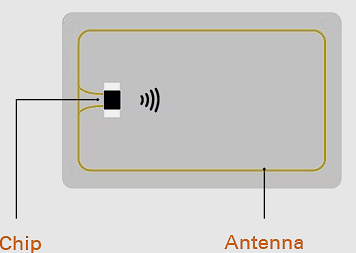
\includegraphics[width=0.4\textwidth]{images/research/emv_card}
    \caption{\centering Структура бесконтактной EMV-карты}
    \label{fig:emv_card}
\end{figure}

С распространением технологии NFC появилась сфера мобильных платежей.
Покупатели получили возможность быстро и безопасно выполнять оплату посредством устройств с поддержкой NFC с помощью виртуальных карт, добавленных в приложение «цифрового кошелька».
Примеры подобных приложений: Apple Pay, Google Pay, Mir Pay и др..


\subsection{Анализ процесса платежа через терминал}

\subsubsection{Оплата бесконтактной картой}

Процесс оплаты с использованием бесконтактной банковской карты может протекать несколькими различными способами.
Как уже было упомянуто ранее, есть онлайн и офлайн оплата через терминал.
Первая происходит с запросом подтверждения банком-эквайера от банка-эмитента в реальном времени.
Вторая происходит исключительно с участием карты и платежного терминала, которые проводит ее аутентификацию.
Также для оплаты могут использоваться разные типы карт.
Однако именно бесконтактную оплату поддерживается только картами, соответствующими стандарту EMV.

При этом карта в защищенной области памяти хранит общий с эмитентом ключ MK-AC (Application Cryptogram Master Key).
Во время совершения оплаты при онлайн-операции карта генерирует на основе MK-AC сессионный ключ SK-AC (Application Cryptogram Session Key) и использует его, данные карты и данные об операции, полученные с терминала, для генерации криптограммы операции ARQC (Authorization Request Cryptogram).
В основе генерации криптограммы лежит алгоритм 3DES (Triple DES).
В общем случае данные по операции поступают от карты к платежному терминалу, далее на хост банка-эквайера, затем к платежной системе и на самом последнем этапе к банку-эмитенту для авторизации.
Результат авторизации передается назад на платежный терминал и карту.
Данный процесс изображен на рисунке~\ref{fig:emv_card_payment}.

\begin{figure}[H]
    \centering
    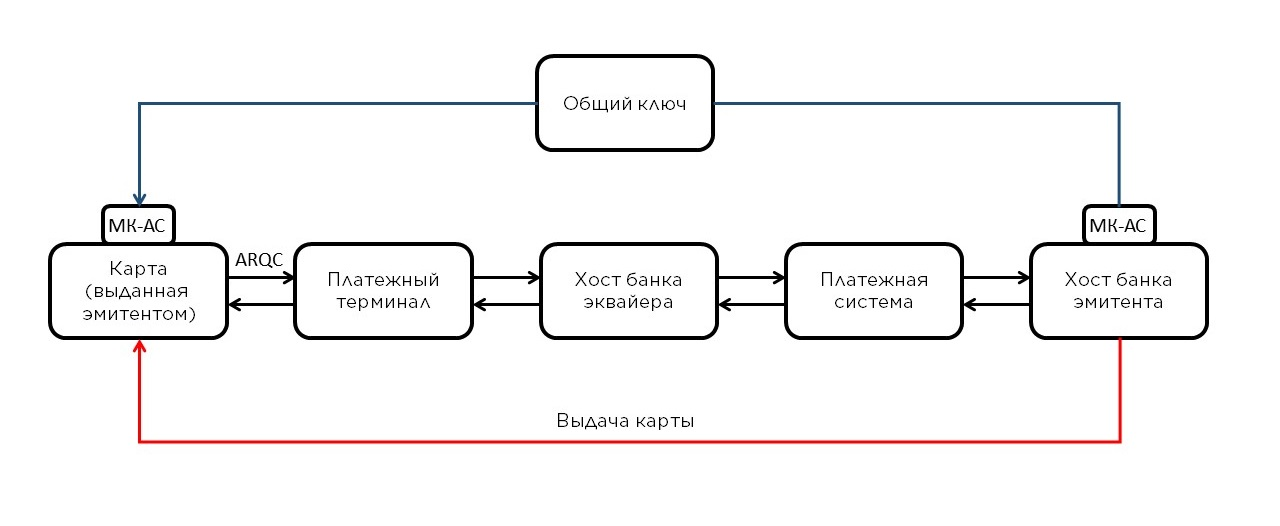
\includegraphics[width=0.8\textwidth]{images/research/emv_card_payment}
    \caption{\centering Процесс оплаты посредством EMV-карты}
    \label{fig:emv_card_payment}
\end{figure}

Банк-эмитент проверяет пришедшую криптограмму операции, путем ее сравнения со значением, которое генерирует сам на основе данных об операции, пришедших вместе с ARQC.
Банк-эмитент может одобрить или отклонить операцию по результатам анализа данных карты, криптограммы, установленных лимитов операций, рисков, а также других параметров~\cite{habr_nspk_mir_payment}.

\subsubsection{Оплата мобильным приложением-кошельком}

При оплате мобильным кошельком выданная банком-эмитентом карта непосредственного участия в оплате не принимает.
Держатель карты вносит данные карты в цифровой кошелек, после чего карта «добавляется» в приложение, точнее не она, а специальный токен-профайл, сгенерированный на базе этой карты.
При этом карточные данные и ключ эмитента MK-AC, хранимый на карте, на телефон не передаются, поэтому оплата посредством приложения происходит с использованием токен-профайла и его специальных ключей.

Процесс добавления карты в приложение-кошелек представлен на рисунке~\ref{fig:add_mob_cardholder}.

\begin{figure}[H]
    \centering
    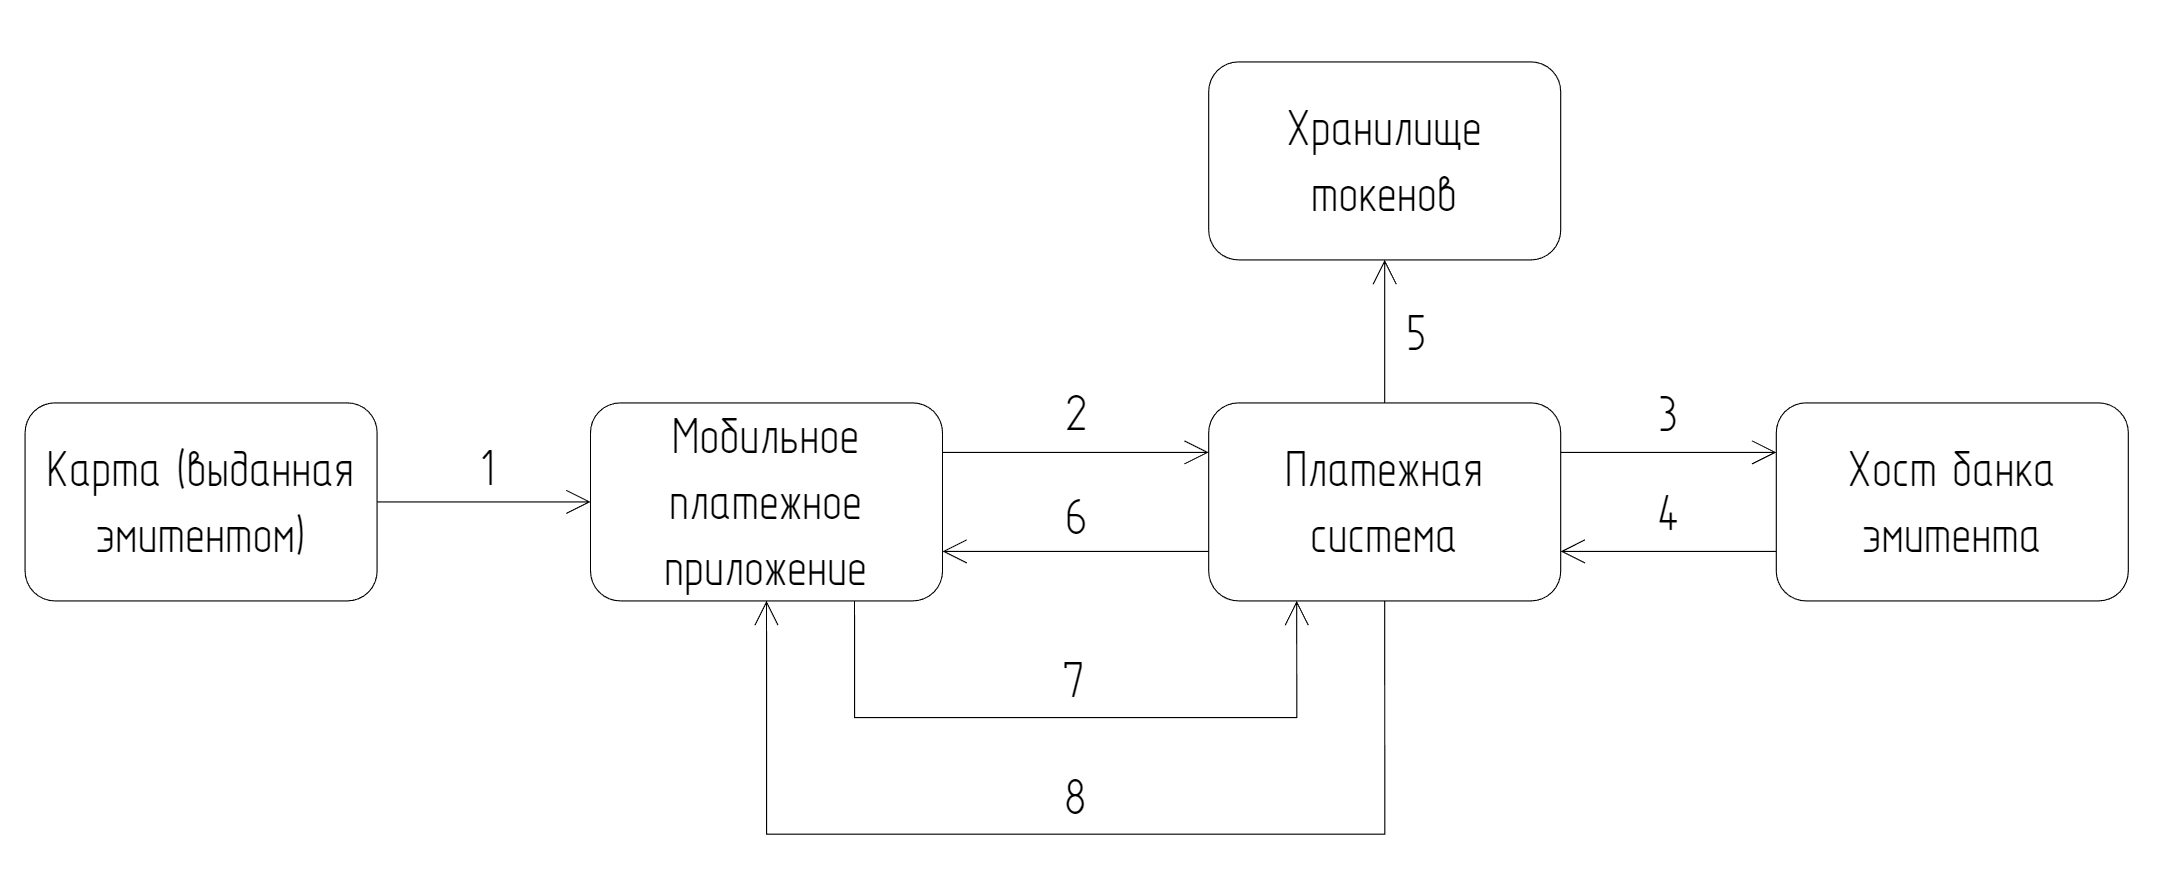
\includegraphics[width=0.8\textwidth]{images/research/add_mob_cardholder}
    \caption{\centering Процесс оплаты посредством мобильного приложения-кошелька}
    \label{fig:add_mob_cardholder}
\end{figure}

Цифрами на рисунке~\ref{fig:add_mob_cardholder} обозначены следующие этапы добавления карты в кошелек:

\begin{enumerate}
    \item держатель карты вводит данные в приложение;
    \item приложение передает их в зашифрованном виде через поставщика услуг мобильного кошелька(WSP~-- Wallet Service Provider) в платежную систему (в случае приложения Mir Pay поставщиком услуг кошелька является НСПК~-- Национальная система платежных карт~-- поэтому данные сразу попадают в ПС);
    \item платформа мобильных платежей (ПМП) производит обработку данных: расшифровывает их, по номеру карты определяет, каким эмитентом она была выдана, и запрашивает у него подтверждение на возможность добавления карты в кошелек;
    \item банк-эмитент возвращает подтверждение или запрет на возможность добавления карты в кошелек;
    \item в случае получения подтверждения для данной карты происходит процедура генерации токен-профайла;
    \item передачи токен-профайла в мобильное приложение пользователя;
    \item мобильное приложение запрашивает у ПМП несколько одноразовых ключей, которые будут использоваться приложением при совершении покупки в качестве сессионных ключей для проведения операции, аналогичных SK-AC.
\end{enumerate}

Таким образом, вместо карточных данных на мобильном устройстве будет храниться токен-профайл, который привязан к конкретным карте и устройству.
Преобразование токен-профайла в исходные данные карты вне платформы мобильных платежей является невозможным.
Одноразовые ключи не могут быть применены более одного раза, поэтому в процессе использования мобильное приложение с некоторой периодичностью подгружает из ПМП новые ключи.


Стоит отметить, что в Mir Pay используется схема, при которой происходит хранение нескольких одноразовых ключей, но существует и другой подход, при котором происходит хранение одного ключа на устройстве.
Такой подход требует наличия аппаратного элементов безопасности (АЭБ) на устройстве, например TEE (Trusted Execution Environment) или SE (Secure Element), и некоторые кошельки применяют именного этот подход, однако он накладывает ограничение в виде наличия АЭБ в устройстве.
Mir Pay также использует АЭБ при его наличии, но уже для хранения одноразовых ключей.

Высокая степень безопасности при использовании приложения гарантируется тем, что для обмена конфиденциальными данными ПМП и Mir Pay генерируют ключевые пары и обмениваются лишь публичными компонентами.
При этом хранением разных ключевых компонент происходит в разных системных хранилищах: как в ключевом хранилище, так и в оперативной памяти.
Для совершения мошеннической операции придется извлечь и расшифровать криптограммы всех ключей, а это неэффективно, в силу того, что для проведения операций используются строго одноразовые ключи.
Передача конфиденциальных данных, например токен-профайла, одноразовых ключей для проведения операций и данных по уже совершенным операциям, начинается только после того, как Mir Pay и ПМП обменялись публичными ключами, создав защищенный канал, и происходит только с использованием <<крипто-стойких>> алгоритмов~\cite{habr_nspk_mir_payment}.

Процесс оплаты с помощью приложения кошелька представлен на рисунке~\ref{fig:emv_mob_payment}.

\begin{figure}[H]
    \centering
    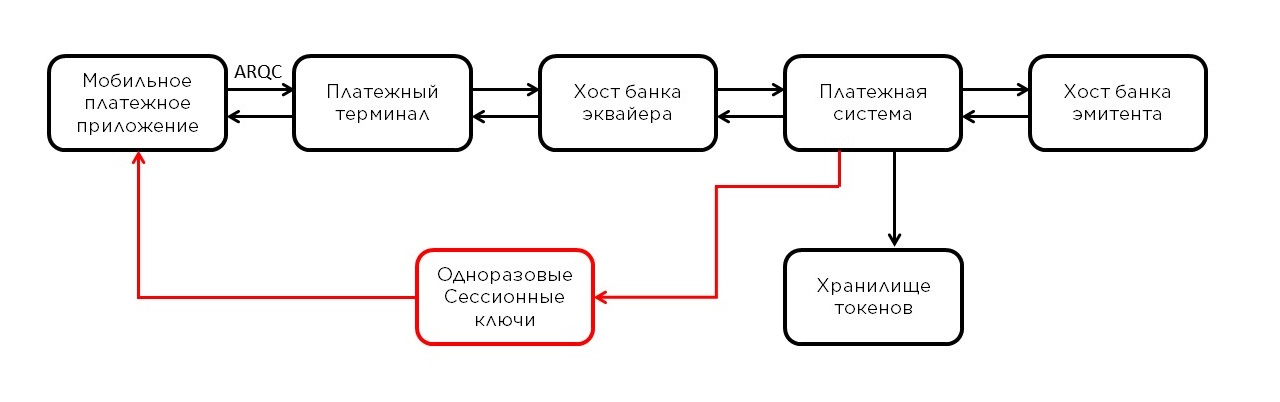
\includegraphics[width=0.8\textwidth]{images/research/emv_mob_payment}
    \caption{\centering Процесс оплаты посредством мобильного приложения-кошелька}
    \label{fig:emv_mob_payment}
\end{figure}

При оплате с помощью мобильного приложения-кошелька используются данные токен-профайла, а криптограмма ARQC генерируется на основе одного из одноразовых ключей (вместо SK-AC как при оплате картой).
Также при оплате приложением может использовать алгоритм шифрования, отличный от 3DES.
В частности в Mir Pay для генерации криптограммы используется более современный симметричный алгоритм блочного шифрования AES (Advanced Encryption Standard).

После генерации ARQC данные об операции так же, как и при оплате банковской картой, проходят через терминал и хост банка-эквайера, попадая в платежную систему.
По наличию токена и его номеру (из токен-профайла) платежная система определяет, что производится полата с помощью мобильного приложения, и направляет данные операции в ПМП для проверки криптограммы и детокенизации~-- превращения токена в данные соответствующей банковской карты.
Данные операции вместе с данными карты отправляются для авторизации в банк-эмитент.
После чего на основе ответа банка-эмитента запускается процесс обратного преобразования платежных данных.

Отличие от оплаты картой как раз в том, что криптограмма проверяется не эмитентом, а ПМП, так как одноразовые ключи и токен-профайл генерируются именно в в платформе мобильных платежей~\cite{habr_nspk_mir_payment}.


\subsection{Анализ платежных технологий}

В предыдущем подразделе были рассмотрены стандартные сценарии выполнения платежных операций.
Отдельное внимание хочется уделить процессам взаимодействия платежного терминала с банковской карты или мобильного платежного приложения и с хостом банка-эквайера.
С целью детального анализа происходящих процессов и используемых в них технологий.

Наиболее важным в данном контексте является стандарт EMV, т.к. он описывает характеристики банковских карт и других средств бесконтактной оплаты, а также весь процесс формирования платежа.

\subsubsection{Стандарт EMV}

\subsubsection{Стандарт ISO/IEC 14443}



\subsection{Анализ существующих решений}

\subsubsection{POS-терминалы}

POS-терминал (от англ.\ Point of Sale, точка продаж)~--- это устройство, предназначенное для приема безналичных платежей с использованием платежных средств, поддерживающих соответствующие терминалу технологии.
POS-терминалы широко используются в розничной торговле, ресторанах, транспорте и других сферах, где требуется осуществление платежей.

Основные функции POS-терминалов:

\begin{itemize}
    \item инициация взаимодействия с платежным средством (карта, смартфон и прочее);
    \item обмен данными с платежным средством, получение данных для формирования транзакции;
    \item связь с банком (напрямую или с помощью устройства-хоста) для авторизации и выполнения транзакций;
    \item выдача чека потребителю (в печатном или электронном виде), возврат ошибки платежа;
    \item обеспечение безопасности платежа, в соответствии со стандартом EMV.
\end{itemize}

POS-терминалы имеют различную структуру, однако можно выделить обобщенную структуру данного устройства.
Она представлена на рисунке~\ref{fig:postrem_struct}.

\begin{figure}[H]
    \centering
    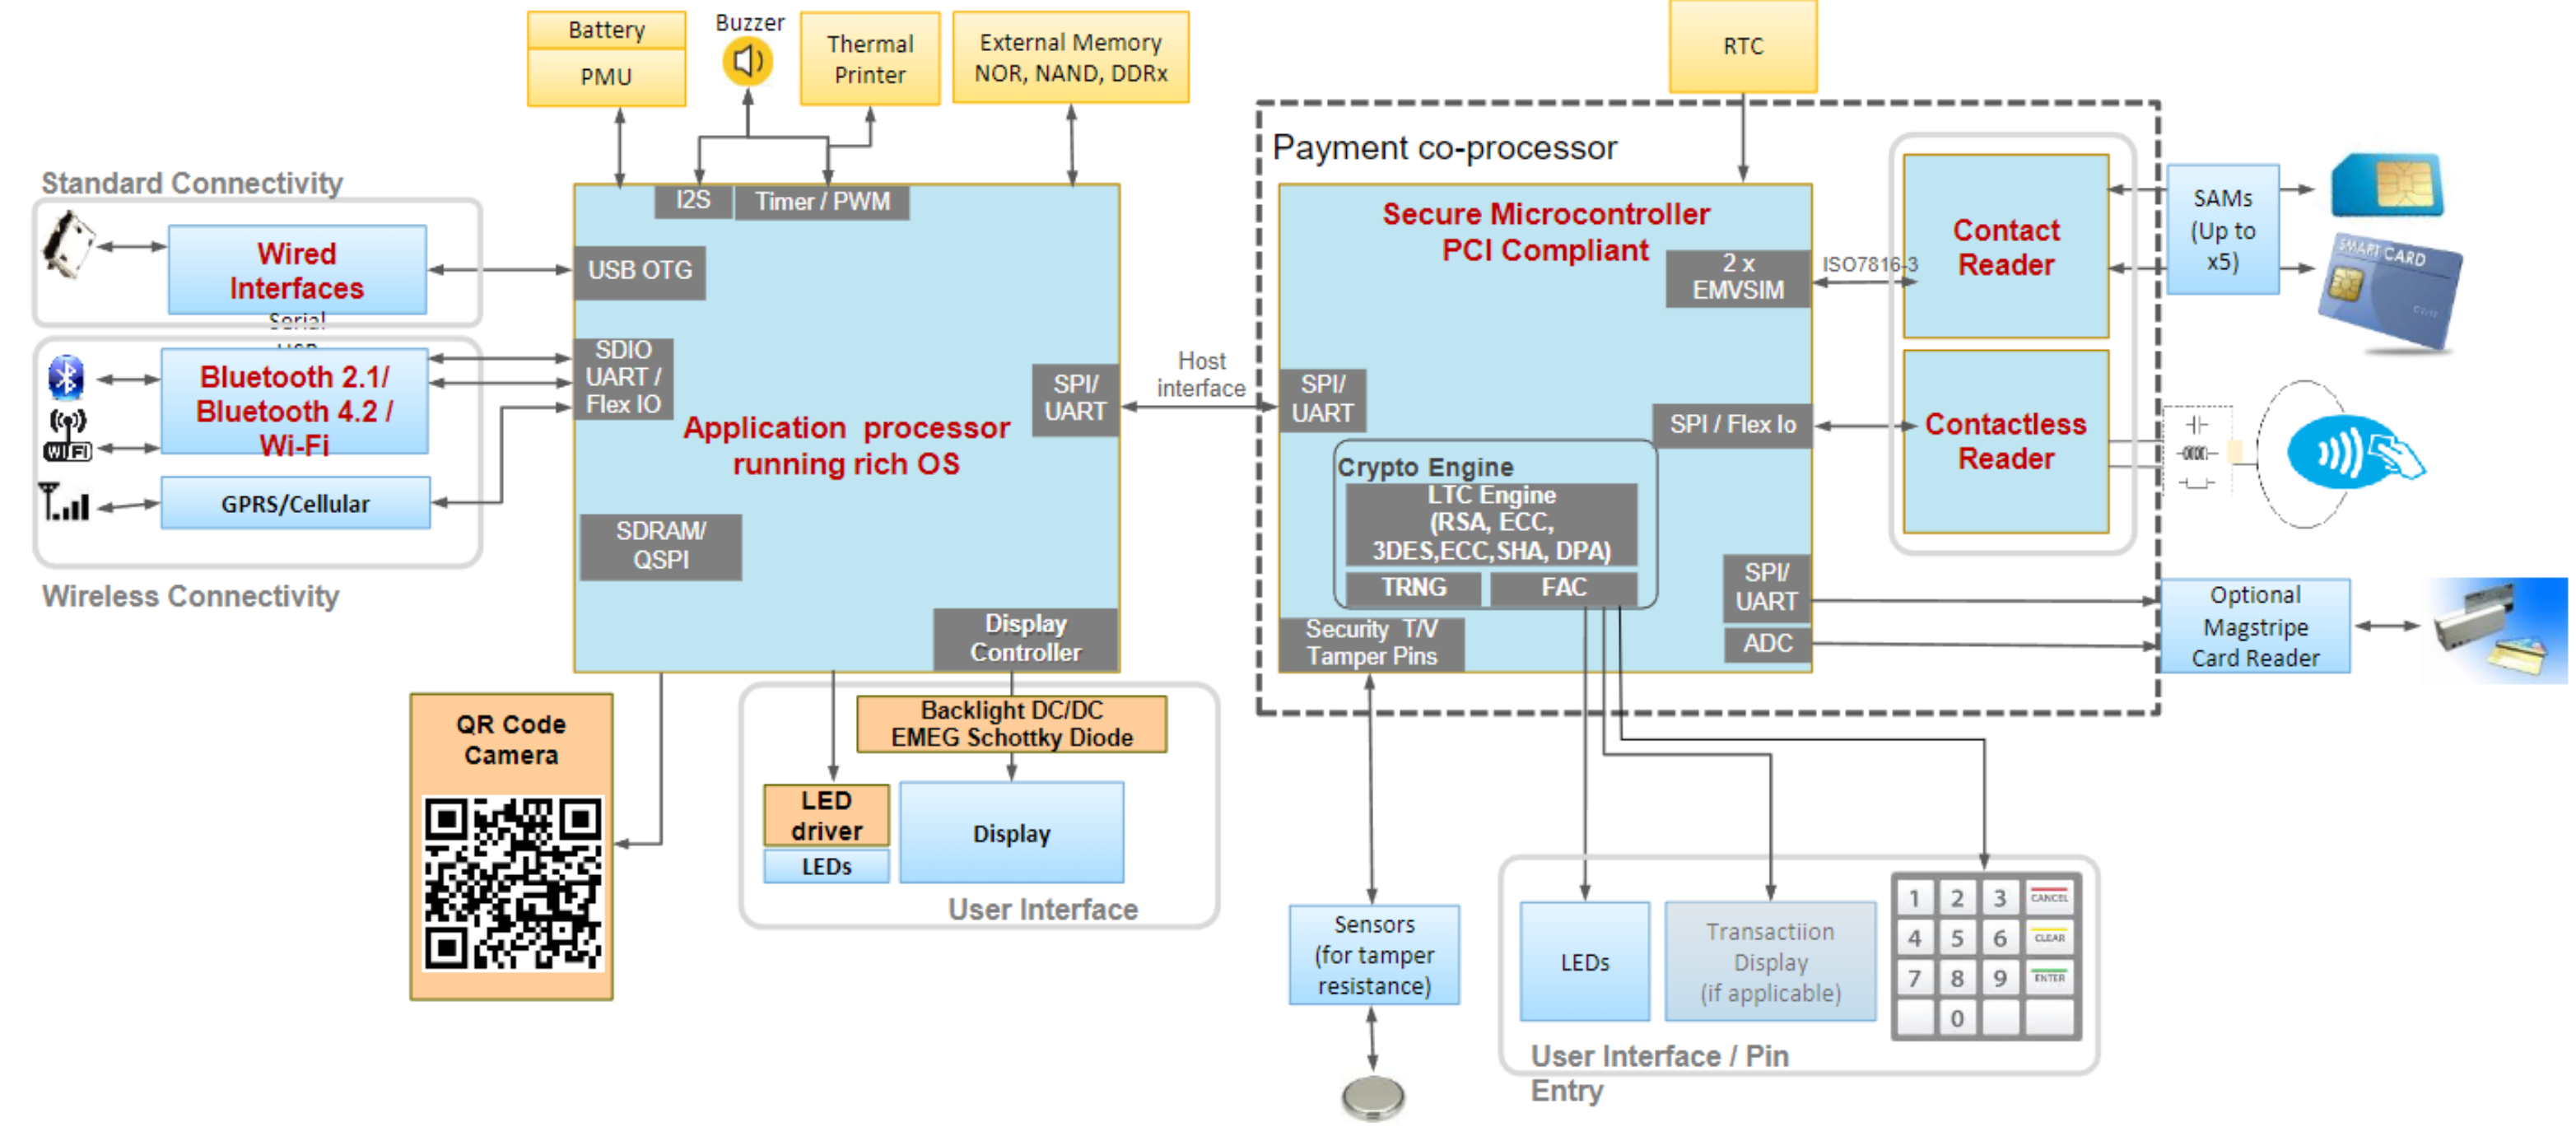
\includegraphics[width=1\textwidth]{images/research/postrem_struct}
    \caption{\centering Распространенная структура POS-терминала}
    \label{fig:postrem_struct}
\end{figure}

К обязательным элементам данного устройства можно отнести следующие:

\begin{itemize}
    \item RFID считыватель для обнаружения и связи со средствами платежа бесконтактным образом;
    \item элемент безопасности (криптографический модуль, SAM-модуль) для сохранения конфиденциальной платежной информации;
    \item модули проводной и/или беспроводной связи для связи с устройством-хостом или прямой связи с банком-эквайером.
\end{itemize}

Стоит отметить, что работа подобного устройства не возможна без программного обеспечения, интегрированного в POS-систему, которое управляет формированием и обработкой транзакций, шифрованием данных, запросами на авторизацию и связь с платежными сетями.

Мобильный эквайринг активно развивается и следствием этого явилось появление mPOS-терминалов и softPOS-терминалов:

\begin{itemize}
    \item mPOS-терминал~-- это портативное устройство, часто смартфон или планшет, оснащенное программным и аппаратным обеспечением, которое позволяет выполнять транзакции;
    \item softPOS терминал~-- это программное решение, с помощью которого мобильное устройство с поддержкой NFC (как правило смартфон или планшет) выступает в роли платежного терминала, т.е. принимает бесконтактные средства платежа, используя встроенный модуль NFC, и осуществляет выполнение платежных транзакций~\cite{pos_term}.
\end{itemize}

Детальное сравнение разновидностей POS-терминалов приведено в таблице~\ref{tab:pos_comparison}.

\begin{table}[H]
    \caption{Сравнение POS, mPOS и SoftPOS терминалов}
    \label{tab:pos_comparison}
    \begin{sloppypar}
        \centering
        \begin{tabularx}{\textwidth}{ | >{\raggedright\arraybackslash}X | >{\raggedright\arraybackslash}X | >{\raggedright\arraybackslash}X | >{\raggedright\arraybackslash}X | }
            \hline
            \textbf{Особенность} & \textbf{POS-терминалы} & \textbf{mPOS-терминалы} & \textbf{SoftPOS-терминалы} \\
            \hline
            Требования к оборудованию & специальные аппаратные компоненты & мобильное устройство с внешним считывателем карт & смартфон или планшет \\
            \hline
            Мобильность & закреплены на торговых точках & могут переносится & могут переносится \\
            \hline
            Методы оплаты & не только бесконтактные платежи & бесконтактные платежи и поддержка приложений цифровых кошельков & бесконтактные платежи и поддержка приложений цифровых кошельков \\
            \hline
            Особенности настройки & необходимость интеграции с сетью и окружением & требуется установка приложения и подключение считывателя карт & только установка приложения \\
            \hline
            Пользовательский интерфейс & отдельный экран устройства & экран мобильного устройства & экран мобильного устройства \\
            \hline
        \end{tabularx}
    \end{sloppypar}
\end{table}


\subsubsection{Сравнение существующих устройств}




\subsection{Формирование требований к системе}


